\section{率失真函数的计算}
\label{sec:rd-computation}

一般的有限概率表没有闭式解。第~\ref{sec:rd-feasible-range}节的三元例子只在$D_{\min}$一点能手算，整条曲线就需要数值方法。式~\eqref{eq:rd-information-rd}是一个凸优化问题，但目标中的$r_q$又依赖$q$，直接求解并不方便。Blahut–Arimoto算法把它拆成两个都有闭式解的子问题，交替求解。本节设$\mathcal{X},\hat{\mathcal{X}}$有限，$p(x)>0$对一切$x$成立（概率为零的源值可以删去），失真矩阵$d(x,\hat{x})$取非负有限值。

\paragraph{用乘子去掉约束}
失真约束先换成罚项。对$s\geq0$，令
\begin{equation}
  F_s^{\star}=\min_{q}\Bigl[I(P_X,q)+s\,\mathbb{E}d(X,\hat{X})\Bigr],
  \label{eq:rd-lagrangian}
\end{equation}
$s$称为失真乘子，单位是bit每单位失真。最小值存在，因为目标在测试信道的紧集上连续。

设$q_s$是一个最小点，$D_s$是它的平均失真。若有平均失真不超过$D_s$而互信息更小的测试信道，它的目标值也更小，与$q_s$最小矛盾。所以$I(P_X,q_s)=R(D_s)$，最小点总落在率失真曲线上。

在码率—失真平面上，目标值为常数$F$的点组成斜率为$-s$的直线$R=F-sD$。求最小就是把这条直线从下方向上平移，直到碰到可行点，第一次碰到的位置就是曲线上斜率为$-s$的切点。图~\ref{fig:rd-ba-curves}(b)画出了三条这样的支撑直线。改变$s$，切点沿曲线移动：$s$大表示失真贵，切点靠近$D_{\min}$；$s$小表示码率贵，切点靠近$D_{\max}$。

\paragraph{两个变量的目标}
困难在于$I(P_X,q)$的分母$r_q$也随$q$变化。把它换成一个自由变量。对$\hat{\mathcal{X}}$上的任一分布$r$（在$r_q>0$处$r>0$），按$\hat{x}$合并后可得
\[
  \sum_{x,\hat{x}}p(x)q(\hat{x}\mid x)\log_2\frac{q(\hat{x}\mid x)}{r(\hat{x})}
  =I(P_X,q)+\sum_{\hat{x}}r_q(\hat{x})\log_2\frac{r_q(\hat{x})}{r(\hat{x})},
\]
最后一项是$D_{\mathrm{KL}}(r_q\Vert r)\geq0$，$r=r_q$时为零。所以互信息是左端对$r$的最小值。

于是令
\begin{equation}
  J(q,r)=\sum_{x}p(x)\sum_{\hat{x}}q(\hat{x}\mid x)\Bigl[\log_2\frac{q(\hat{x}\mid x)}{r(\hat{x})}+s\,d(x,\hat{x})\Bigr],
  \label{eq:rd-ba-objective}
\end{equation}
则$F_s^{\star}=\min_{q,r}J(q,r)$。对两个变量交替求最小，每一步都有闭式解。

\paragraph{固定$r$求$q$}
引入
\begin{equation}
  Z_r(x)=\sum_{\hat{x}}r(\hat{x})\,2^{-s\,d(x,\hat{x})},\qquad
  w_r(\hat{x}\mid x)=\frac{r(\hat{x})\,2^{-s\,d(x,\hat{x})}}{Z_r(x)}.
  \label{eq:rd-ba-q-update}
\end{equation}
$w_r(\cdot\mid x)$是一个概率分布：把当前的重构边缘乘以失真的指数权重$2^{-sd}$，再归一化。由$s\,d=-\log_2(2^{-sd})$，式~\eqref{eq:rd-ba-objective}方括号中的量可以写成
\[
  \log_2\frac{q(\hat{x}\mid x)}{r(\hat{x})2^{-s\,d(x,\hat{x})}}=\log_2\frac{q(\hat{x}\mid x)}{w_r(\hat{x}\mid x)}-\log_2Z_r(x).
\]
代回去，得到
\[
  J(q,r)=\sum_{x}p(x)\,D_{\mathrm{KL}}\bigl(q(\cdot\mid x)\Vert w_r(\cdot\mid x)\bigr)-\sum_{x}p(x)\log_2Z_r(x).
\]
KL散度非负且只在两分布相同时为零，所以固定$r$时最优的$q$恰是$w_r$，最小值为
\begin{equation}
  J(w_r,r)=-\sum_{x}p(x)\log_2Z_r(x).
  \label{eq:rd-ba-j-value}
\end{equation}

式~\eqref{eq:rd-ba-q-update}有直观的含义：给定$x$，一个重构值被选中的机会正比于两件事的乘积，一是它在当前方案中被用到的频率$r(\hat{x})$，二是它离$x$有多近。失真每增加$1$，权重就乘以$2^{-s}$。

\paragraph{固定$q$求$r$}
由前面的分解，固定$q$时最优的$r$就是$r_q$，即式~\eqref{eq:rd-output-marginal}。把两步合起来，新的重构边缘是
\begin{equation}
  r^{\mathrm{new}}(\hat{x})=\sum_{x}p(x)\,w_r(\hat{x}\mid x)=r(\hat{x})\,c_r(\hat{x}),\qquad
  c_r(\hat{x})=\sum_{x}\frac{p(x)\,2^{-s\,d(x,\hat{x})}}{Z_r(x)} .
  \label{eq:rd-ba-r-update}
\end{equation}
$c_r(\hat{x})$是一个乘性修正因子：大于$1$的重构值在新方案中被用得更多。由$Z_r$的定义，
\[
  \sum_{\hat{x}}r(\hat{x})c_r(\hat{x})=\sum_{x}\frac{p(x)}{Z_r(x)}\sum_{\hat{x}}r(\hat{x})2^{-s\,d(x,\hat{x})}=\sum_xp(x)=1,
\]
所以$r^{\mathrm{new}}$仍是概率分布，且$\max_{\hat{x}}c_r(\hat{x})\geq1$。若某个$r(\hat{x})=0$，它以后永远为零，因此初值必须处处为正。

\paragraph{计算过程}
下面结合同一个例子写出计算过程。仍取$X\sim\operatorname{Bern}(0.3)$与Hamming失真，乘子取$s=\log_29\approx3.170$，于是一次错误的权重是$2^{-s}=\tfrac19$。由第~\ref{sec:rd-binary}节，$R'(D)=-\log_2\frac{1-D}{D}$，斜率为$-\log_29$的点是$D=0.1$，所以算法应收敛到$R(0.1)\approx0.4123$，目标最优值为
\[
  F_s^{\star}=R(0.1)+0.1\log_29\approx0.4123+0.3170=0.7293 .
\]

\needspace{6\baselineskip}
\paragraph{变量}
\begin{itemize}
  \item $\bm{A}$：$\lvert\mathcal{X}\rvert\times\lvert\hat{\mathcal{X}}\rvert$矩阵，元素$a_{x,\hat{x}}=2^{-s\,d(x,\hat{x})}$，计算一次后不变。例中$\bm{A}=\begin{bmatrix}1&1/9\\1/9&1\end{bmatrix}$。
  \item $r$：长度$\lvert\hat{\mathcal{X}}\rvert$的概率向量，当前重构边缘$r^{(t)}$。
  \item $Z$：长度$\lvert\mathcal{X}\rvert$的向量，归一化常数$Z^{(t)}(x)$。
  \item $q$：$\lvert\mathcal{X}\rvert\times\lvert\hat{\mathcal{X}}\rvert$矩阵，本轮的测试信道$q^{(t+1)}$，每行和为$1$。
  \item $c$：长度$\lvert\hat{\mathcal{X}}\rvert$的修正因子。
  \item $J^{(t+1)}$与$\epsilon^{(t+1)}$：本轮目标值与最优性误差界，用于停止判断；$D^{(t+1)}$与$I^{(t+1)}$：本轮测试信道的平均失真与互信息，用于报告结果。
\end{itemize}

\paragraph{初始化}
$r^{(0)}$取处处为正的分布，常用均匀分布；给定停止容差$\varepsilon>0$与最大轮数。例中
\[
  r^{(0)}=(0.5,\,0.5),\qquad \varepsilon=10^{-3}.
\]

\needspace{6\baselineskip}
\paragraph{每轮更新}
第$t+1$轮（$t=0,1,\dots$）：
\begin{enumerate}
  \item \textbf{归一化常数。}按式~\eqref{eq:rd-ba-q-update}，取$r=r^{(t)}$算出$Z^{(t)}(x)$，即矩阵$\bm{A}$的第$x$行与$r^{(t)}$的内积。例中第一轮
  \[
    Z^{(0)}(0)=0.5+\frac{0.5}{9}=\frac59,\qquad Z^{(0)}(1)=\frac{0.5}{9}+0.5=\frac59 .
  \]

  \item \textbf{测试信道。}按式~\eqref{eq:rd-ba-q-update}，$q^{(t+1)}$的第$x$行是$r^{(t)}$与$\bm{A}$第$x$行的逐元素乘积除以$Z^{(t)}(x)$。例中第一轮
  \[
    \begin{gathered}
    q^{(1)}(0\mid0)=\frac{0.5}{5/9}=0.9,\qquad q^{(1)}(1\mid0)=0.1,\\
    q^{(1)}(1\mid1)=0.9,\qquad q^{(1)}(0\mid1)=0.1 ,
    \end{gathered}
  \]
  正是第~\ref{sec:rd-test-channels}节以$0.1$翻转的测试信道。

  \item \textbf{目标值。}由式~\eqref{eq:rd-ba-j-value}，$J^{(t+1)}=-\sum_xp(x)\log_2Z^{(t)}(x)$。例中第一轮
  \[
    J^{(1)}=-\log_2\frac59\approx0.8480 .
  \]

  \item \textbf{修正因子与新边缘。}按式~\eqref{eq:rd-ba-r-update}算$c$与$r^{(t+1)}=r^{(t)}c$。例中第一轮
  \[
    c(0)=\frac{0.7\times1+0.3\times\frac19}{5/9}=1.32,\qquad c(1)=\frac{0.7\times\frac19+0.3\times1}{5/9}=0.68,
  \]
  \[
    r^{(1)}=(0.5\times1.32,\ 0.5\times0.68)=(0.66,\ 0.34).
  \]

  \item \textbf{误差界与停止。}令$\epsilon^{(t+1)}=\max_{\hat{x}}\log_2c(\hat{x})$。下面的定理~\ref{thm:rd-ba-bounds}说明最优值被夹在$J^{(t+1)}-\epsilon^{(t+1)}$与$J^{(t+1)}$之间。若$\epsilon^{(t+1)}\leq\varepsilon$则停止，否则进入下一轮。例中第一轮
  \[
    \epsilon^{(1)}=\log_21.32\approx0.4005,
  \]
  所以$F_s^{\star}\in[0.4475,\,0.8480]$，继续。

  \item \textbf{报告量。}按式~\eqref{eq:rd-test-distortion}与式~\eqref{eq:rd-test-information}算$q^{(t+1)}$的平均失真$D^{(t+1)}$与互信息$I^{(t+1)}$。例中第一轮
  \[
    D^{(1)}=0.1,\qquad I^{(1)}\approx0.4558 .
  \]
\end{enumerate}

第二轮从$r^{(1)}=(0.66,0.34)$出发：
\[
  Z^{(1)}(0)=0.66+\frac{0.34}{9}\approx0.6978,\qquad Z^{(1)}(1)=\frac{0.66}{9}+0.34\approx0.4133 .
\]
测试信道变为$q^{(2)}(1\mid0)\approx0.0541$，$q^{(2)}(0\mid1)\approx0.1774$，错误开始向罕见符号转移。目标值与修正因子为
\[
  J^{(2)}\approx0.7458,\qquad c\approx(1.0838,\ 0.8373),\qquad r^{(2)}\approx(0.7153,\ 0.2847),
\]
误差界$\epsilon^{(2)}\approx0.1161$，报告量$D^{(2)}\approx0.0911$，$I^{(2)}\approx0.4468$。

此后各轮的结果列在表~\ref{tab:rd-ba-rounds}中。误差界每轮约缩小为原来的$0.4$倍，第$7$轮的误差界约为$1.2\times10^{-3}$，第$8$轮约为$5.1\times10^{-4}$，首次低于$\varepsilon$，停止。最终得到
\[
  \begin{gathered}
  q^{(8)}(1\mid0)\approx0.0358,\qquad q^{(8)}(0\mid1)\approx0.2495,\\
  D^{(8)}\approx0.0999,\qquad I^{(8)}\approx0.4125 ,
  \end{gathered}
\]
与精确解$q(1\mid0)=\tfrac1{28}\approx0.0357$、$q(0\mid1)=0.25$、$(D,R)=(0.1,0.4123)$相差不到$10^{-3}$。

\begin{BookInlineTable}
  \centering
  \caption{Blahut–Arimoto算法在例中的各轮结果，$s=\log_29$，$r^{(0)}=(0.5,0.5)$。$r^{(t)}(1)$是本轮更新后的重构边缘，其余各量由本轮开始时的边缘$r^{(t-1)}$算出。}
  \label{tab:rd-ba-rounds}
  \begin{tabular}{cccccc}
    \toprule
    $t$ & $r^{(t)}(1)$ & $J^{(t)}$ & $\epsilon^{(t)}$ & $D^{(t)}$ & $I^{(t)}$ \\
    \midrule
    $1$ & $0.3400$ & $0.8480$ & $0.4005$ & $0.1000$ & $0.4558$ \\
    $2$ & $0.2847$ & $0.7458$ & $0.1161$ & $0.0911$ & $0.4468$ \\
    $3$ & $0.2642$ & $0.7318$ & $0.0408$ & $0.0951$ & $0.4288$ \\
    $4$ & $0.2559$ & $0.7297$ & $0.0160$ & $0.0978$ & $0.4196$ \\
    $5$ & $0.2525$ & $0.7294$ & $0.0066$ & $0.0990$ & $0.4155$ \\
    $6$ & $0.2511$ & $0.7293$ & $0.0028$ & $0.0996$ & $0.4137$ \\
    $7$ & $0.2505$ & $0.7293$ & $0.0012$ & $0.0998$ & $0.4129$ \\
    $8$ & $0.2502$ & $0.7293$ & $0.0005$ & $0.0999$ & $0.4125$ \\
    \bottomrule
  \end{tabular}
\end{BookInlineTable}

\paragraph{误差界}
停止条件依赖一个可计算的最优性误差界。它来自对任意测试信道成立的一个下界。

\begin{theorem}[Blahut–Arimoto的上下界]
\label{thm:rd-ba-bounds}
对任一处处为正的分布$r$，记$Z_r,w_r,c_r$如式~\eqref{eq:rd-ba-q-update}与式~\eqref{eq:rd-ba-r-update}。则对任意测试信道$q$，
\begin{equation}
  I(P_X,q)+s\,\mathbb{E}_qd\geq-\sum_{x}p(x)\log_2Z_r(x)-\sum_{\hat{x}}r_q(\hat{x})\log_2c_r(\hat{x}),
  \label{eq:rd-ba-lower}
\end{equation}
因而
\begin{equation}
  -\sum_xp(x)\log_2Z_r(x)-\max_{\hat{x}}\log_2c_r(\hat{x})\leq F_s^{\star}\leq-\sum_xp(x)\log_2Z_r(x).
  \label{eq:rd-ba-bounds}
\end{equation}
\end{theorem}

\begin{proof}
由$J$的分解，取$r=r_q$时$J(q,r_q)=I(P_X,q)+s\,\mathbb{E}_qd$。下面用$w_r$改写$J(q,r_q)$。由$w_r$的定义，$2^{s\,d}=r/(w_rZ_r)$，于是
\[
  \log_2\frac{q(\hat{x}\mid x)\,2^{s\,d(x,\hat{x})}}{r_q(\hat{x})}
  =\log_2\frac{q(\hat{x}\mid x)}{w_r(\hat{x}\mid x)}+\log_2\frac{r(\hat{x})}{r_q(\hat{x})}-\log_2Z_r(x).
\]
按$p(x)q(\hat{x}\mid x)$求和，左端是$I(P_X,q)+s\,\mathbb{E}_qd$，右端第三项给出$-\sum_xp(x)\log_2Z_r(x)$，第二项给出$-D_{\mathrm{KL}}(r_q\Vert r)$。

第一项对每个$\hat{x}$用引理~\ref{lem:rd-log-sum}，以$a_x=p(x)q(\hat{x}\mid x)$、$b_x=p(x)w_r(\hat{x}\mid x)$合并$x$：
\[
  \sum_{x,\hat{x}}p(x)q(\hat{x}\mid x)\log_2\frac{q(\hat{x}\mid x)}{w_r(\hat{x}\mid x)}
  \geq\sum_{\hat{x}}r_q(\hat{x})\log_2\frac{r_q(\hat{x})}{r(\hat{x})c_r(\hat{x})},
\]
这里用了式~\eqref{eq:rd-ba-r-update}：$w_r$的输出边缘是$rc_r$。右端等于$D_{\mathrm{KL}}(r_q\Vert r)-\sum_{\hat{x}}r_q(\hat{x})\log_2c_r(\hat{x})$。

三项相加，$D_{\mathrm{KL}}(r_q\Vert r)$恰好抵消，得到式~\eqref{eq:rd-ba-lower}。右端最后一项不超过$\max_{\hat{x}}\log_2c_r(\hat{x})$，对$q$取最小即得式~\eqref{eq:rd-ba-bounds}的左半。右半来自$w_r$本身的目标值：它不小于$F_s^{\star}$，又不超过$J(w_r,r)$，而后者由式~\eqref{eq:rd-ba-j-value}给出。
\end{proof}

误差界$\max_{\hat{x}}\log_2c_r(\hat{x})$为零，当且仅当所有$c_r(\hat{x})\leq1$；由$\sum_{\hat{x}}rc_r=1$，这时在$r>0$处$c_r=1$，$r$是更新的不动点。所以$\epsilon$同时度量“离不动点多远”与“离最优值多远”。

\paragraph{收敛}
误差界说明了何时可以停止，但没有说明它一定会变小。下面的定理给出目标值的收敛速度。

\begin{theorem}[目标值的收敛]
\label{thm:rd-ba-convergence}
设初值$r^{(0)}$处处为正，按上面的两步交替迭代，$J^{(t)}$是由$r^{(t-1)}$按式~\eqref{eq:rd-ba-j-value}算出的目标值。设$q^{\star}$是式~\eqref{eq:rd-lagrangian}的一个最小点，$r^{\star}=r_{q^{\star}}$。则$J^{(t)}$非增，并且
\begin{equation}
  J^{(T)}-F_s^{\star}\leq\frac{D_{\mathrm{KL}}(r^{\star}\Vert r^{(0)})}{T},\qquad T=1,2,\dots .
  \label{eq:rd-ba-rate}
\end{equation}
\end{theorem}

\begin{proof}
\emph{单调。}$J^{(t+1)}$是$J(\cdot,r^{(t)})$的最小值，$r^{(t)}$又是$J(q^{(t)},\cdot)$的最小点，所以
\[
  J^{(t+1)}=\min_qJ(q,r^{(t)})\leq J(q^{(t)},r^{(t)})\leq J(q^{(t)},r^{(t-1)})=J^{(t)}.
\]

\emph{每轮的进展。}在式~\eqref{eq:rd-ba-lower}中取$q=q^{\star}$与$r=r^{(t)}$，左端是$F_s^{\star}$，于是
\[
  J^{(t+1)}-F_s^{\star}\leq\sum_{\hat{x}}r^{\star}(\hat{x})\log_2c_{r^{(t)}}(\hat{x}).
\]
由式~\eqref{eq:rd-ba-r-update}，$c_{r^{(t)}}=r^{(t+1)}/r^{(t)}$。初值处处为正，而$2^{-sd}>0$使每个$c$为正，所以各$r^{(t)}$处处为正，右端可以写成
\[
  \sum_{\hat{x}}r^{\star}(\hat{x})\log_2\frac{r^{(t+1)}(\hat{x})}{r^{(t)}(\hat{x})}
  =D_{\mathrm{KL}}(r^{\star}\Vert r^{(t)})-D_{\mathrm{KL}}(r^{\star}\Vert r^{(t+1)}).
\]

\emph{求和。}对$t=0,\dots,T-1$相加，右端逐项相消，
\[
  \sum_{t=1}^{T}\bigl(J^{(t)}-F_s^{\star}\bigr)\leq D_{\mathrm{KL}}(r^{\star}\Vert r^{(0)})-D_{\mathrm{KL}}(r^{\star}\Vert r^{(T)})\leq D_{\mathrm{KL}}(r^{\star}\Vert r^{(0)}).
\]
由单调性，左端每一项都不小于$J^{(T)}-F_s^{\star}$，于是得到式~\eqref{eq:rd-ba-rate}。
\end{proof}

初值处处为正保证$D_{\mathrm{KL}}(r^{\star}\Vert r^{(0)})$有限；若某个最优重构值的初始概率为零，它永远回不来，算法可能停在非最优点。由$F_s^{\star}\leq I^{(t)}+sD^{(t)}\leq J^{(t)}$，所报告测试信道的目标值也以同样的速度逼近最优值；再由测试信道集合的紧性与目标的连续性，$q^{(t)}$的每个极限点都是最小点。

例中$r^{\star}=(0.75,0.25)$，
\[
  D_{\mathrm{KL}}(r^{\star}\Vert r^{(0)})=0.75\log_21.5+0.25\log_20.5\approx0.1887 .
\]
式~\eqref{eq:rd-ba-rate}保证第$8$轮的误差不超过$0.024$，实际误差只有约$4\times10^{-7}$。图~\ref{fig:rd-ba-iterations}显示，这个例子中误差按几何速度下降，比$1/T$快得多；$1/T$是对一切有限概率表都成立的保证，几何速度则依赖具体问题。

\begin{BookInlineFigure}
  \centering
  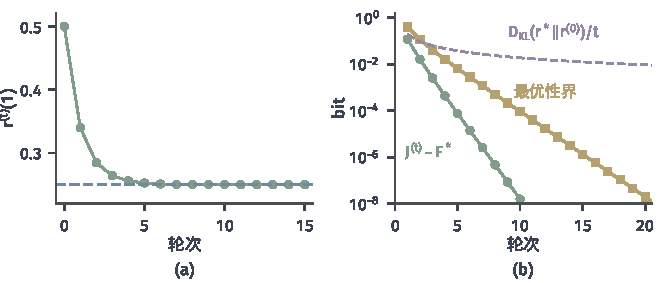
\includegraphics[width=112mm]{figures/07-probability/05-source-coding/matplotlib/rd-ba-iterations/figure.pdf}
  \caption{Blahut–Arimoto算法在例中的收敛，$s=\log_29$，$r^{(0)}=(0.5,0.5)$。(a)重构边缘$r^{(t)}(1)$（绿），蓝色虚线是极限$0.25$。(b)对数刻度下的目标误差$J^{(t)}-F_s^{\star}$（绿）、可计算的误差界$\epsilon^{(t)}=\max\log_2c$（黄）与定理~\ref{thm:rd-ba-convergence}的保证$D_{\mathrm{KL}}(r^{\star}\Vert r^{(0)})/t$（紫色虚线）。}
  \label{fig:rd-ba-iterations}
\end{BookInlineFigure}

\paragraph{改变乘子描出曲线}
每个$s$只给出曲线上的一个点$(D^{(t)},I^{(t)})$，失真不是事先指定的。要得到整条曲线，就对一列$s$分别运行；要求指定$D$处的$R(D)$，就利用$D_s$随$s$增大而不增，对$s$作二分。图~\ref{fig:rd-ba-curves}(a)对$24$个$s$运行算法，所得的点都落在式~\eqref{eq:rd-binary}的曲线上。

\begin{BookInlineFigure}
  \centering
  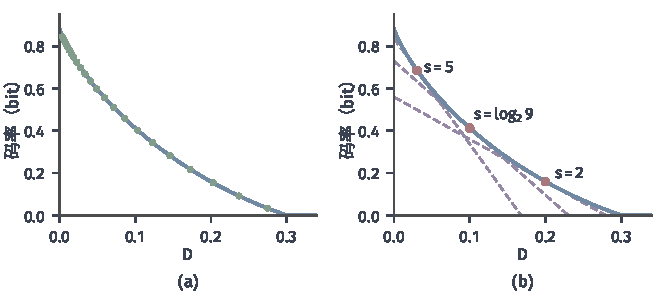
\includegraphics[width=112mm]{figures/07-probability/05-source-coding/matplotlib/rd-ba-curves/figure.pdf}
  \caption{改变乘子描出$\operatorname{Bern}(0.3)$与Hamming失真的率失真曲线。(a)$s$从$1.4$到$8$等距取$24$个值，算法的输出（绿点）落在闭式曲线$h_2(0.3)-h_2(D)$（蓝）上。(b)$s=2,\log_29,5$时目标的等值线$R=F_s^{\star}-sD$（紫色虚线）是曲线的支撑直线，红点是切点$D_s=1/(1+2^{s})$。}
  \label{fig:rd-ba-curves}
\end{BookInlineFigure}

$s$很小时，码率极贵，最优点停在零码率处。例中曲线在$D_{\max}=0.3$左侧的斜率是$-\log_2\frac{0.7}{0.3}\approx-1.222$，所以$s\leq1.222$时最小点是$(0.3,0)$；这时迭代中$r^{(t)}(1)$缓慢趋于零，收敛变慢。$s\to\infty$时切点趋于$D_{\min}$，但对有限的$s$一般到不了端点。$R(D_{\min})$可以另算：只允许把每个$x$送到使$d(x,\cdot)$最小的重构值，在这个子集上最小化互信息，这是同一类型、失真项消失的问题；第~\ref{sec:rd-feasible-range}节的三元例子就是这样算出$0.6$的。

\paragraph{线性区段}
若$R(D)$在某个区间$[D_1,D_2]$上是直线，斜率为$-s_0$，则$s=s_0$时这一段上的所有点都使式~\eqref{eq:rd-lagrangian}最小，算法收敛到哪一个取决于初值，改变$s$也只会在两个端点之间跳跃。这时先用略大和略小于$s_0$的乘子求出两个端点的测试信道，中间的点用它们的混合得到：由引理~\ref{lem:rd-mi-convex}，混合信道的互信息不超过弦的高度，而在线性区段上弦就是曲线本身。在块编码中，这对应于两种码的分时。反过来，曲线在某点有折角时，一段$s$都对应同一个点，二分得到的$D_s$会在这里停留。

\paragraph{计算代价}
每轮要算$Z$、$q$、$c$，各需$O(\lvert\mathcal{X}\rvert\lvert\hat{\mathcal{X}}\rvert)$次运算，存储$\bm{A}$与$q$需要同样大小的空间。数值上，$s$很大时$2^{-sd}$可能下溢，常把每行的指数减去该行的最小失真再计算，归一化后结果不变。还需注意算法求出的是信息率失真函数及其测试信道。它告诉我们极限是多少，以及随机码本应按什么边缘生成，但不给出有限块长的编码器。
